\documentclass[11pt,a4paper]{article}
\usepackage{fontspec}
\setmainfont{chinese.ttf}[Path=fonts/,BoldFont=chinese.ttf,BoldFeatures={FakeBold=1.5},ItalicFont=chinese.ttf,ItalicFeatures={FakeSlant=0.15}]
\XeTeXlinebreaklocale "zh"
\XeTeXlinebreakskip=0pt plus 1pt minus 0.5pt
\renewcommand{\abstractname}{摘要}\renewcommand{\refname}{参考文献}\renewcommand{\figurename}{图}\renewcommand{\tablename}{表}
\usepackage[margin=24mm]{geometry}
\usepackage{amsmath,amssymb,booktabs,tabularx,graphicx,array,placeins}
\usepackage[colorlinks=true,allcolors=black]{hyperref}
\hypersetup{pdftitle={来源隔离评估揭示文献催化机器学习的泛化缺口},
  pdfauthor={Zhang Junyu and Li Wenjie},
  pdfcreator={XeLaTeX}}
\setlength{\parskip}{2pt}
\emergencystretch=3em
\newcommand{\pp}{\,pp}
\newcommand{\mgg}{\,mg\,h$^{-1}$\,g$_{\mathrm{cat}}^{-1}$}

\title{\textbf{来源隔离评估揭示文献催化机器学习的泛化缺口：\\
少标签适配、输入表征与公开研究复现审计}}
\author{张君宇\quad 李文杰\\[2pt]
\small 中国石油大学（华东）机电工程学院，青岛 266580}
\date{2026年9月28日}

\begin{document}
\maketitle

\begin{abstract}
\noindent
文献衍生催化数据具有出版来源异质性，记录级随机划分的性能是否代表未见来源泛化，以及少量新来源标签能恢复多少性能，需要分开评估。
我们提出来源隔离、按标签预算索引、逐来源配对并带负对照的评测框架，研究两个反应体系、四个目标：
1,245条甲醇转化率/选择性成对记录、1,230条甲醇时空收率（STY）记录及1,794条甲烷氧化偶联（OCM）记录。
整泄漏组留出使四目标合并$R^2$比随机记录划分下降0.20--0.47。
五条标签可恢复可观误差，例如原始协议中局部岭将甲醇转化率来源等权MAE从5.279降至2.429\pp{}。
配对表征与标签排列区分来源水平和真实输入--响应对应；后续强本地、残差与混合对照进一步识别历史响应的增量。
同五标签、同冻结混合器的查询V选样使STY误差从62.608降至50.274、OCM F1从3.081降至2.708，
分别改善19.7\%和12.1\%，均通过原五面板家族校正。
91个额外文献来源和一个含1,739条测量的实测家族扩展了应用证据，后者组成选样在19/20次身份分离划分中改善。
最后，两项公开工作流的原协议结果可恢复；Suvarna受控对照的$R^2$从0.876降至0.319，
Xu后续同五折配对复核的来源等权MAE从69.620升至126.365（原生STY单位）。
研究将来源泛化缺口、标签辅助恢复、表征与测量覆盖，以及公开研究审计连接为同一证据链。
\end{abstract}

\section{引言}
催化机器学习的训练数据很少来自专门设计的实验，而是汇编自已发表的文献：每篇论文报告
少量测量值，各自带有其催化剂制备、表征习惯、原料纯度与报道惯例。TheMeCat
\cite{toldy}、三十年甲醇合成回顾 \cite{yan}、Suvarna等的时空收率数据集
\cite{suvarna} 与Schmack等的氧化偶联荟萃分析 \cite{schmack} 使这种数据模式
变得可行，基于此类语料的模型也常规报告很高的精度。

\paragraph{两个不同的泛化问题。}文献语料的随机记录级划分回答一个合法但特定的问题：
模型对\emph{已见来源的新记录}内插得多好？同一出版物的记录共享装置、催化剂族与报道
惯例，随机划分会把训练记录的近重复放到测试侧。部署真正关心的问题——\emph{模型对
从未见过的文献来源表现如何？}——由来源隔离评估回答：整个出版物（或上游溯源相同的
记录组）被整体留出。学习理论预言源域精度不约束目标域误差 \cite{bendavid}，
分组重采样是聚类数据的标准补救 \cite{roberts}；催化场景缺少的是跨目标、跨反应
体系的量化缺口，以及对能做什么的评估。

\paragraph{少标签适配是实际的应对。}拟合好的模型遇到新文献来源时，实践者有介于
"信模型"与"全面补实验"之间的便宜选择：从新来源收集少量带标签记录做适配。均值偏移、
带惩罚仿射、经验贝叶斯收缩 \cite{efron} 与局部回归都是经典工具；多元
校准模型的迁移在化学计量学中有长期历史 \cite{feudale}。缺少的是按预算索引、
防泄漏的账目：$k$条标签时每个适配器买到多少、对照强简单基线、逐来源配对、带负对照。

\paragraph{诊断适配利用了什么。}均值偏移只能修来源级平移；特征依赖的局部模型还能
利用来源内的标签—输入对应。二者机制不同、含义不同，平均误差的配对区间无法区分。
我们因此加入标签置换诊断，并用同批记录的严格配对表征对照追问输入表征本身是否
限制了适配能发现的东西。

\paragraph{公开研究审计。}这一现象不应是我们自己基准的偶然。我们所依赖的两个语料
源自数据与代码公开的已发表研究；我们复现这些工作流并对其实施同样的来源隔离压力测试。

\paragraph{贡献。}本文有四项贡献。(i)~文献衍生催化数据的评测框架：泄漏组上的来源
隔离外层折、标签盲固定测试集、$k\in\{0,1,2,3,5,10\}$的标签预算与嵌套校准前缀、
强简单适配器、逐来源配对与负对照。(ii)~两个反应体系四个目标上记录级乐观偏差的
定量证据，含零标签行为与完整少标签适配曲线。(iii)~少标签适配利用了什么的诊断——
来源级平移对比真实标签—输入对应——含严格配对的表征实验，表明表征同时改变基础模型
与适配收益的性质。(iv)~两项开放已发表工作流的复现审计，区分close reproduction与
受控划分对照。后续强本地对照、同预算选样、额外来源和身份划分增强上述证据链；经典估计器和V最优设计本身不作为新算法贡献。

\section{相关工作}
聚类数据的分组/分块重采样是标准做法 \cite{roberts}；近期的催化基准比较了
按化学式分组与随机交叉验证 \cite{wu}。域适应理论区分源精度与目标误差
\cite{bendavid}。我们评估的适配估计器皆为经典：均值偏移与仿射再校准是标准实践
\cite{steyerberg2019}，经验贝叶斯收缩源自Efron与Morris \cite{efron}，
多元校准迁移在化学计量学中已有综述 \cite{feudale}。我们构建所依赖的语料为
TheMeCat \cite{toldy}、Communications Engineering甲醇回顾 \cite{yan}、
Schmack等的OCM荟萃分析 \cite{schmack} 与Suvarna等的STY研究 \cite{suvarna}。
这些来源均未将带标签预算的来源隔离评估作为主要协议；定位与原始协议细节见补充材料A。

\section{数据}\label{sec:data}
\subsection{数据来源}
表\ref{tab:data}汇总四个语料。四个目标来自两个反应体系。甲醇语料（1{,}245条成对
记录、82源、80泄漏组）提供CO$_2$转化率与甲醇选择性（百分点），由TheMeCat v1
\cite{toldy} 与Communications Engineering回顾数据集 \cite{yan} 组合；STY
语料（1{,}230条、109源）源自Suvarna等公开数据集 \cite{suvarna}（CC BY 4.0），
与转化率语料重叠20个出版物标识，故按同反应异目标任务处理；OCM语料（1{,}794条、
408源、405泄漏组）来自Schmack等荟萃分析 \cite{schmack}，提供C$_2$收率
（百分点）。目标绝不跨单位比较。

\begin{table}[t]
\centering\small
\caption{语料、目标与队列。"主队列"=校准池支持完整$k\le10$曲线的来源（固定测试集
$\max(5,\lceil n/4\rceil)$条记录）。}
\label{tab:data}
\begin{tabularx}{\linewidth}{lXXXX}
\toprule
 & CO$_2$转化率 & 甲醇选择性 & 甲醇STY & OCM C$_2$收率 \\
\midrule
记录数 & \multicolumn{2}{c}{1{,}245（成对）} & 1{,}230 & 1{,}794 \\
来源数 & \multicolumn{2}{c}{82} & 109 & 408 \\
泄漏组数 & \multicolumn{2}{c}{80} & 109 & 405 \\
主队列 & \multicolumn{2}{c}{32} & 28 & 22 \\
单位 & \multicolumn{2}{c}{pp} & mg\,h$^{-1}$g$_{cat}^{-1}$ & pp \\
特征族 & \multicolumn{4}{l}{工况描述符（甲醇另含SBET；OCM F1另含所记录组成）} \\
许可 & \multicolumn{4}{l}{CC BY 4.0（TheMeCat、OCM补充材料、STY数据集）} \\
\bottomrule
\end{tabularx}
\end{table}

\subsection{数据重建与纳入标准}
甲醇语料从两份上游文件逐行重建（表\ref{tab:ledger}）：1{,}124+500原始行经在任何
结果查看前固定的规则筛选为748+497条成对记录——两条目标均在$[0,100]$内报告；温度、
压力、H$_2$/CO$_2$为正且已报告；GHSV与BET允许缺失、在训练折内填补；不做任何基于
表现的筛选；真实零响应保留；全字段上游重复只保留一份，条件与目标相同但组成不同者
保留为不同测量。每条排除逐行留档。二十条早期内部版本按$10^{\mathrm{LN}}$重建BET的
记录改由存储的自然对数字段按$\exp(\mathrm{LN})$重算并留有日志。OCM语料对荟萃分析
补充材料施行同一哲学（1{,}802条原始记录、412个出版物编号；参考表缺失或歧义的条目
按行级日志剔除，三对同引用来源合并）。

\begin{table}[t]
\centering\small
\caption{甲醇语料构建台账。排除记录逐行保留在排除清单中；无任何基于表现的筛选。}
\label{tab:ledger}
\begin{tabular}{lrr}
\toprule
 & TheMeCat v1 & CommsEng MeOH \\
\midrule
上游文件行数 & 1{,}124 & 500 \\
纳入的成对记录 & 748 & 497 \\
无成对目标 & $-319$ & --- \\
恰缺一条目标 & $-26$ & --- \\
归属未定/DOI无效 & $-30$ & $-3$ \\
全字段上游重复 & $-1$ & --- \\
\bottomrule
\end{tabular}
\end{table}

\subsection{来源身份与泄漏组}
来源是DOI可标识的出版物条目，不是实验室：同一课题组的两篇论文计为两个来源，一篇
论文可能跨多种催化剂。历史主语料的物理催化剂身份未被恢复，因而不据此声称对新物理家族的泛化；额外实测家族的报告身份划分另见第5.6节。引用规范化后相同、或完整上游测量相同的记录并入同一泄漏组；泄漏组是
一切外层划分的原子，任何组都不跨训练/测试两侧。OCM来源编号是上游荟萃分析的映射
而非DOI，且含部分标识不统一的参考文献与专利；这作为局限保留。

\subsection{单位统一与缺失}
甲醇特征覆盖：温度433--673~K、压力0.4--80 bar、H$_2$/CO$_2$ 1--10、GHSV
0.87--240~L\,g$^{-1}$h$^{-1}$（缺失6.2\%）、BET 2--975~m$^2$g$^{-1}$（缺失18.5\%）；
目标0--59.6\%与0--100\%。OCM：温度773--1223~K、CH$_4$分压0.009--2.7 bar、O$_2$
0.003--1.35 bar、CH$_4$/O$_2$ 0.8--38.3、总压0.11--4.5 bar、接触时间0.0017--182.5~s
（缺失2.5\%）；C$_2$收率0--37.0\%。STY：特征无缺失；STY 0.74--2620
mg\,h$^{-1}$g$_{cat}^{-1}$。一切填补均为当前训练折的中位数。GHSV参考态与惰性定义
未逐篇对齐——数值一致不代表定义一致，这作为局限保留而非悄悄修复。

\subsection{OCM F0/F1表征配对}
OCM审计表对每条模型行记录催化剂标识与上游表的出版物编号；把所记录组成关联到模型
行是身份关联（催化剂编号+出版物编号一对一，零未匹配，目标值核对相等）。F0为仅
工况表征（六个描述符）。F1加入所记录组成：至多4个阳离子与2个载体槽位，按角色分开
编码，含"被列出"指示、已知mol分数合计、每物种缺失含量计数与显式未见物种通道，词表
只在当前训练分区拟合（钠不作缺失标记；未列出是"未报告"，不是证明不存在；mol分数合计只编码已报告值（论文常省略平衡组分），并非归一化组成）。F0与F1
共享行身份、标签、来源、泄漏组、外层折、$T/U/A$索引、校准顺序与模型选择程序；
因此该对比是严格配对的流程比较，不是加入组成的因果效应。


\subsection{额外文献来源与实测实验家族}
扩展证据沿用同一来源隔离原则。Mine等发布的OCM更新汇编\cite{mine}经完整历史参考文献筛查，
删除三个重新列入的旧来源，按热催化条件、有效实测响应、单位和组成模式纳入2,381条记录、91个额外出版来源；
其中52个来源支持完整随机查询预算曲线，40个支持高温查询。历史预处理、模型和超参数均先于这些目标来源的支持与查询计分冻结。
文献来源不重叠构成出版条目层面的扩展验证，并不等同于实验室独立。

另一项应用来自Nishimura等的作者实测文件\cite{nishimura2023new}。
2,928行原始记录经阶段筛选、必要响应与温度检查和重复催化剂--条件去重后，保留1,739条测量、116个报告催化剂编号。
五个验证阶段仍属于一个出版来源、一个实验家族。缺少的四项工况和组成用量沿冻结预处理的缺失处理执行，不推测物理值。
除普通查询外，初始身份留出及20次完整身份分离划分每次把29个催化剂编号放入查询、87个放入支持池，
同一编号的全部记录仅在一侧。重复划分描述该家族内的查询组成敏感性。


\section{评测协议}\label{sec:protocol}
\begin{figure}[t]
\centering
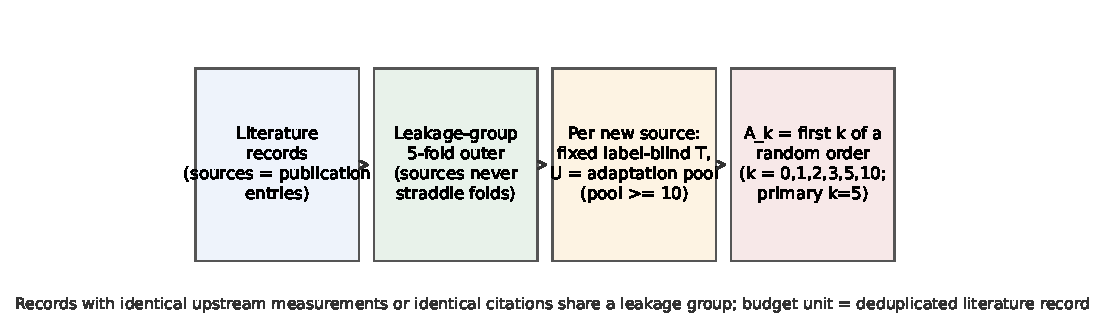
\includegraphics[width=\linewidth]{figs/fig1_design.pdf}
\caption{评测设计。泄漏组按五个外层种子各分五折；每组每种子恰被测试一次。来源内部
由固定随机划分给出标签盲测试集$T$，剩余池$U$随机排序，$A_k$取前$k$项，
$A_1\subset A_2\subset A_3\subset A_5\subset A_{10}$。所有适配器共享同一$T$、同一
顺序与同一基础模型。}
\label{fig:design}
\end{figure}
每个外层种子$s\in\{42,101,202,303,404\}$下泄漏组分五折；每折内基础模型（岭
$\alpha\in\{0.1,1,10,100\}$与梯度提升树$n\in\{100,300\}\times$深度$\in\{2,3\}$
外加一项深配置，由内层来源组交叉验证按内层等权MAE选出）在训练来源上拟合、预测全部
留出行。每个留出来源内，标签盲固定测试集$T$（$\max(5,\lceil n/4\rceil)$条）被评分，
剩余池$U$随机排序，$A_k$取前$k$项；每来源抽五十次校准顺序。主预算$k=5$；$k=1$与
$k=10$为指定次要预算。所有适配器共享同一$T$、同一顺序、同一基础预测与同一外层
划分；测试来源信息从不进入模型选择、先验拟合或填补。

\paragraph{适配器。}皆为强简单基线，非新算法。记基础预测$p$、校准标签$(y_A,p_A)$、
测试预测$p_T$：目标均值/中位数不用模型；均值偏移加$\overline{y_A-p_A}$，修来源级
残差均值；带惩罚仿射允许残差与中心化预测之间的斜率关系，惩罚在训练来源上拟合；
经验贝叶斯把观测偏移向训练来源折外残差估计的先验收缩，保护单标签校准；局部岭回归
在$(x_A,y_A)$上以训练侧特征变换重拟合，利用来源内特征—标签对应。另保留仅温度的
岭回归。

\paragraph{指标。}主指标为来源等权MAE：来源内部先对$T$、再对校准重复平均绝对误差，
最后跨来源等权平均。行加权MAE与合并$R^2$（默认预测平均）连同显式单位一并报告；
重复校准抽取绝不被当作独立来源。不确定性为泄漏组聚类自助（100{,}000次、种子基
510{,}927），条件于已拟合模型——是经验性来源间区间，不是训练全流程的重采样。基础基准未作多重比较校正；非主对比为描述性。后续选样分析另保留其预定的比较家族校正，见下文。

\paragraph{负对照。}打乱标签与打乱预测对照属主协议；专门的alignment诊断
（\ref{sec:perm}节）对每个$A_k$的标签抽二十次均匀随机置换、先逐置换计损失再平均。
这是回顾性诊断，不是正式置换检验，也不是部署规则。


\paragraph{扩展预测对照与历史响应复用。}
在原有强简单基线之外，扩展对照纳入仅温度岭回归、残差岭回归、收缩混合及历史调参的本地径向基函数（RBF）模型。
记冻结历史预测为$f_G$，有标签支持集为$S$，查询集为$Q$。本地岭回归直接拟合$(z_S,y_S)$；
残差岭回归拟合$y_S-f_G(S)$后加回$f_G(Q)$。对相同正则化、自由截距的线性拟合算子$R_{S,\alpha}$，
\begin{equation}\label{eq:ext_projection}
q_R(Q)-q_L(Q)=f_G(Q)-R_{S,\alpha}[f_G(S)](Q).
\end{equation}
该分解识别支持拟合未能重建的历史响应成分；匹配正则化的消融单独保留。
收缩混合$q_M=(1-w)q_L+wq_R$以支持集留一预测和历史伪来源先验确定$w$，不使用查询标签。
RBF及扩展工况/组成分块核也只由允许的历史数据调参。完整公式和所有变体见补充材料B。

\paragraph{同预算测量位置与表征交叉。}
面向查询的V最优设计贪心降低指定查询输入上的工作方差\cite{yubi,gorodetsky2016}。
随机、覆盖、面向池的V、核V和稳健多视图V为对照；在主要选样比较中，标签预算和部署预测器参数固定。
同一实际支持集分别交给F0和F1预测器，并另设仅打乱选样化学信息行对应的对照。
历史学习的对比协方差、自适应视图门控、分块核、中心化平方/绝对风险及协方差平均风险的完整比较均保留，
用于区分表征、预测器复杂度与选样规则的作用，而不以增加组件数量替代效果比较。

\paragraph{预测算子与风险敏感性。}
固定自由截距核预测器可写为$\widehat y_Q=Ay_S$、$A\mathbf1=\mathbf1$。
在给定工作协方差$\Sigma_0$下，令$B=[-A\ I]$，平方风险为
$\mathcal R_0=|Q|^{-1}\operatorname{tr}(B\Sigma_0B^\top)$。
若$\|\Sigma-\Sigma_0\|_2\le\varepsilon$，已有分析给出
\begin{equation}\label{eq:ext_bound}
|\mathcal R_\Sigma-\mathcal R_0|\le
\varepsilon\left(1+\frac{\|A\|_F^2}{|Q|}\right).
\end{equation}
它解释标签噪声放大和查询任务依赖性；给定半径的协方差界不是实际MAE保证。推导和惩罚消融见补充材料B。

\paragraph{分析层与推断口径。}
基础基准与扩展全因子分析保留各自冻结的历史拟合、适配参数和支持顺序。
因此，同一面板的未适配或随机支持点估计在不同分析层可略有不同；每项增量均在本层匹配对照内计算，
不跨层相减。原始基准区间保持原统计口径；扩展五面板主要选样家族采用校正区间，
其余信息干预和已打开实测家族分析保留探索性/开发性状态。来源数、重复种子数和催化剂划分数分别报告。


\section{结果}\label{sec:results}
\subsection{记录级与来源隔离评估（研究问题1）}
\begin{figure}[t]
\centering
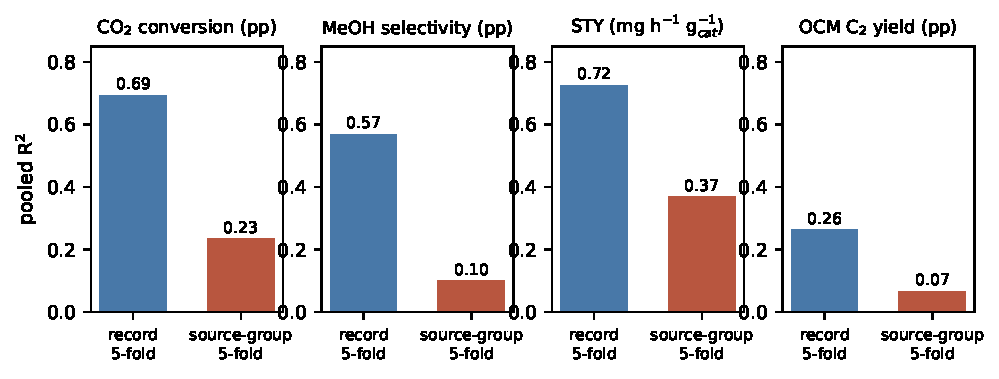
\includegraphics[width=\linewidth]{figs/fig2_split_contrast.pdf}
\caption{记录级与来源组五折对比（固定模型与种子；两种模式每条记录每种子恰测一次）。
合并$R^2$差距：0.460（转化率）、0.469（选择性）、0.356（STY）、0.196（OCM）。}
\label{fig:split}
\end{figure}
记录、特征与固定模型完全相同时，划分方式的影响超过我们测试的任何协变量选择
（图\ref{fig:split}）：整泄漏组留出而非随机留出时，四个目标的合并$R^2$分别下降
0.460、0.469、0.356、0.196。两种设计回答不同的泛化问题——语料内插值与新来源迁移
——我们作描述性报告，不解读为泄漏的因果估计。此后所有结果均用来源组划分。

\subsection{零标签行为与来源漂移（研究问题2之始）}
在全部合格来源的留出行上（仅无标签方法），基础模型的来源等权MAE在每个目标都优于
训练均值常数：5.88对6.33\pp{}、20.33对21.63\pp{}、5.47对5.82\pp{}、136.6对187.2~\mgg{}。
主队列内排序依赖面板：基础模型在甲醇转化率（5.279对5.910\pp{}）与STY（135.1对
164.8~\mgg{}）上获胜，但OCM上训练均值略优（5.177对5.285\pp{}）——与\ref{sec:repr}节
量化的表征限制一致。面板绝不混用。

\subsection{跨预算的少标签适配（研究问题2、3）}
\begin{figure}[t]
\centering
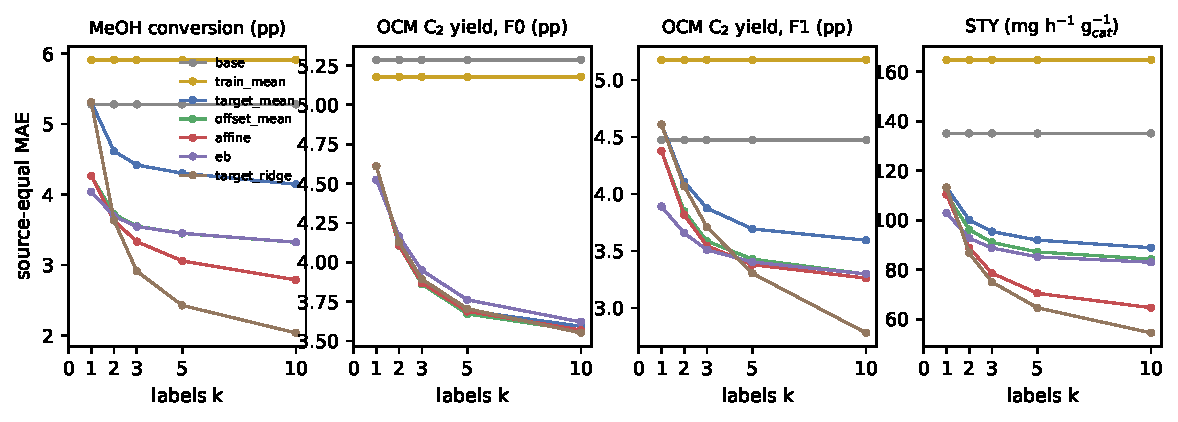
\includegraphics[width=\linewidth]{figs/fig3_learning_curves.pdf}
\caption{主队列学习曲线（随机选择器；来源等权MAE；$k=0$来自同一固定$T$）。单位
逐面板不同，绝不跨面板比较。}
\label{fig:curves}
\end{figure}
\begin{table}[t]
\centering\small
\caption{主队列、主预算$k=5$、随机选择器：来源等权MAE（不截断主预测；点估计；完整95\%区间见补充材料A及数值登记）。单位：pp；STY为mg\,h$^{-1}$g$_{cat}^{-1}$。}
\label{tab:k5}
\begin{tabular}{lcccc}
\toprule
方法 & 转化率(pp) & 选择性(pp) & OCM F0(pp) & STY \\
\midrule
base（无标签） & 5.279 & 22.736 & 5.285 & 135.115 \\
训练均值 & 5.910 & 24.167 & 5.177 & 164.803 \\
目标均值 & 4.304 & 17.136 & 3.693 & 91.993 \\
目标中位数 & 4.443 & 18.100 & 3.817 & 92.259 \\
均值偏移 & 3.450 & 15.748 & 3.672 & 87.225 \\
仿射 & 3.060 & 12.540 & 3.688 & 70.508 \\
经验贝叶斯 & 3.452 & 15.990 & 3.762 & 85.244 \\
局部岭回归 & \textbf{2.429} & \textbf{11.547} & 3.705 & \textbf{64.660} \\
\bottomrule
\end{tabular}
\end{table}
表\ref{tab:k5}与图\ref{fig:curves}给出主预算结果。五条标签买到大幅下降，但赢家随
任务而异。甲醇转化率上局部岭回归把基础误差降54\%（5.28$\to$2.43\pp{}），仿射至
3.06\pp{}；STY上局部岭回归再度主导（64.7~\mgg{} 对目标均值92.0）。OCM-F0上所有适配器
落在目标均值0.15\pp{}内（3.67--3.82），局部岭回归（3.705）并不优于目标均值（3.693）。
逐源配对对比（表\ref{tab:paired}）表明平均值与频繁的逐源受损并存：$k=1$时均值偏移
使15/32（转化率）与17/32（选择性）个来源变差，EB收缩把两目标的受损数都降到11/32
而不抬高平均。$k=10$时局部岭回归改善32/32与29/32个来源（转化率/选择性）。三种
$R^2$口径与完整方法集（15方法、双选点、双预算）见补充材料。

\begin{table}[t]
\centering\small
\caption{主队列逐源配对对比：平均MAE差（方法$-$参照，pp）与$k=1,5,10$时32源中的
改善数（随机选择器）。负差有利于方法。}
\label{tab:paired}
\begin{tabular}{llrrr}
\toprule
目标 & 比较 & $k=1$ & $k=5$ & $k=10$ \\
\midrule
CO$_2$转化率 & EB对base & $-1.24$（21/32） & $-1.83$（23/32） & $-1.95$（24/32） \\
 & 仿射对均值偏移 & 0（构造） & $-0.39$（25/32） & $-0.53$（24/32） \\
 & 局部岭对EB & $+1.27$（8/32） & $-1.02$（25/32） & $-1.29$（28/32） \\
\midrule
甲醇选择性 & EB对base & $-3.87$（21/32） & $-6.75$（20/32） & $-7.20$（20/32） \\
 & 仿射对均值偏移 & 0（构造） & $-3.21$（22/32） & $-3.89$（22/32） \\
 & 局部岭对EB & $+2.35$（7/32） & $-4.44$（21/32） & $-5.49$（23/32） \\
\bottomrule
\end{tabular}
\end{table}


\subsubsection{扩展强对照：区分来源水平、本地关系与历史响应}
表\ref{tab:ext_information}将预测器比较扩展到九类方法，并补全OCM F1。
在该匹配的扩展协议中，F1的来源等权MAE由未适配模型4.527降到支持均值3.693、本地岭3.374、残差岭3.109和混合3.081\pp{}。
STY对应的全局、支持均值、本地岭与混合误差为139.258、91.993、65.210和62.608\mgg{}。
这延伸了原始预算曲线的结论：少量目标响应既能估计来源水平，也能提供有用的输入--响应关系。
历史响应复用的增量须与使用相同标签的本地模型比较，不能全部归因于历史知识迁移。
\begin{table}[htbp]\centering\footnotesize
\setlength{\tabcolsep}{4pt}
\caption{扩展信息对照，五标签随机支持。每个面板内共享支持与查询。该表的冻结拟合和支持顺序独立于基础基准表\ref{tab:k5}；不跨表计算增益。STY保留原生单位，其余为百分点。}\label{tab:ext_information}
\begin{tabular}{lrrrrr}
\toprule
方法 & 转化率 & 选择性 & OCM F0 & OCM F1 & STY \\
\midrule
历史模型 & 5.271 & 22.740 & 5.302 & 4.527 & 139.258 \\
新来源均值 & 4.304 & 17.136 & 3.693 & 3.693 & 91.993 \\
均值偏移 & 3.455 & 15.747 & 3.672 & 3.423 & 88.265 \\
仿射校正 & 3.083 & 12.539 & 3.694 & 3.360 & 71.225 \\
经验贝叶斯偏移 & 3.457 & 15.988 & 3.759 & 3.415 & 86.510 \\
局部岭回归 & 2.429 & 11.547 & 3.655 & 3.374 & 65.210 \\
仅温度岭回归 & 2.519 & 11.535 & 3.677 & 3.677 & 87.098 \\
残差岭回归 & 2.720 & 12.077 & 3.701 & 3.109 & 69.889 \\
收缩组合 & 2.441 & 11.584 & 3.660 & 3.081 & 62.608 \\
\bottomrule
\end{tabular}

\end{table}

\subsubsection{额外来源验证与同预算测量位置}
在额外文献的52个完整曲线来源中，F1全局、支持均值、本地岭和混合的五标签随机查询MAE分别为
6.120、4.490、3.593和3.552\pp{}（表\ref{tab:ext_external}）。40来源的高温查询结果同表报告，保持不同查询总体分开。
额外来源延续了标签辅助条件校准的价值；它不以新增出版条目的数量替代实验室独立性。
\begin{table}[htbp]\centering\footnotesize
\setlength{\tabcolsep}{4pt}
\caption{额外文献来源上的五标签冻结应用。随机查询52源，高温查询40源；F0/F1为同一记录集的配对表征。MAE单位为百分点。}\label{tab:ext_external}
\begin{tabular}{lrrrr}
\toprule
方法 & F0随机查询 & F1随机查询 & F0高温查询 & F1高温查询 \\
\midrule
历史模型 & 5.973 & 6.120 & 5.699 & 5.140 \\
新来源均值 & 4.490 & 4.490 & 5.556 & 5.556 \\
均值偏移 & 4.502 & 4.606 & 5.512 & 5.397 \\
仿射校正 & 4.284 & 4.410 & 5.209 & 5.328 \\
经验贝叶斯偏移 & 4.545 & 4.621 & 5.205 & 4.942 \\
局部岭回归 & 4.045 & 3.593 & 4.801 & 4.365 \\
仅温度岭回归 & 3.779 & 3.779 & 4.697 & 4.697 \\
残差岭回归 & 4.421 & 3.716 & 5.375 & 4.454 \\
收缩组合 & 4.054 & 3.552 & 4.806 & 4.335 \\
\bottomrule
\end{tabular}

\end{table}

当预算与冻结混合器保持不变，查询V选样使STY从62.608降到50.274\mgg{}、OCM F1从3.081降到2.708\pp{}，
分别对应19.7\%和12.1\%的点估计误差降低（表\ref{tab:ext_acquisition}）。两项通过原五面板家族校正，
说明不仅标签数量重要，测量位置也决定同一预算的利用效率。其他面板的结果一并保留。
\begin{table}[htbp]\centering\footnotesize
\setlength{\tabcolsep}{4pt}
\caption{同五标签、同冻结混合器下的查询V对随机选样。来源数逐面板列出；校正区间为原生单位的MAE差，而非误差比的区间。}\label{tab:ext_acquisition}
\begin{tabular}{lrrrrl}\toprule 预测任务 & $n$ & 随机 & 查询V选样 & 误差降低(\%) & 校正后差值区间\\\midrule
转化率 & 32 & 2.441 & 2.121 & 13.1 & [-0.707, 0.068]\\
选择性 & 32 & 11.584 & 10.683 & 7.8 & [-2.140, 0.615]\\
STY & 28 & 62.608 & 50.274 & 19.7 & [-25.965, -2.874]\\
OCM F0 & 22 & 3.660 & 3.768 & -3.0 & [-0.355, 0.714]\\
OCM F1 & 22 & 3.081 & 2.708 & 12.1 & [-0.746, -0.056]\\
\bottomrule\end{tabular}

\end{table}
\begin{figure}[htbp]\centering
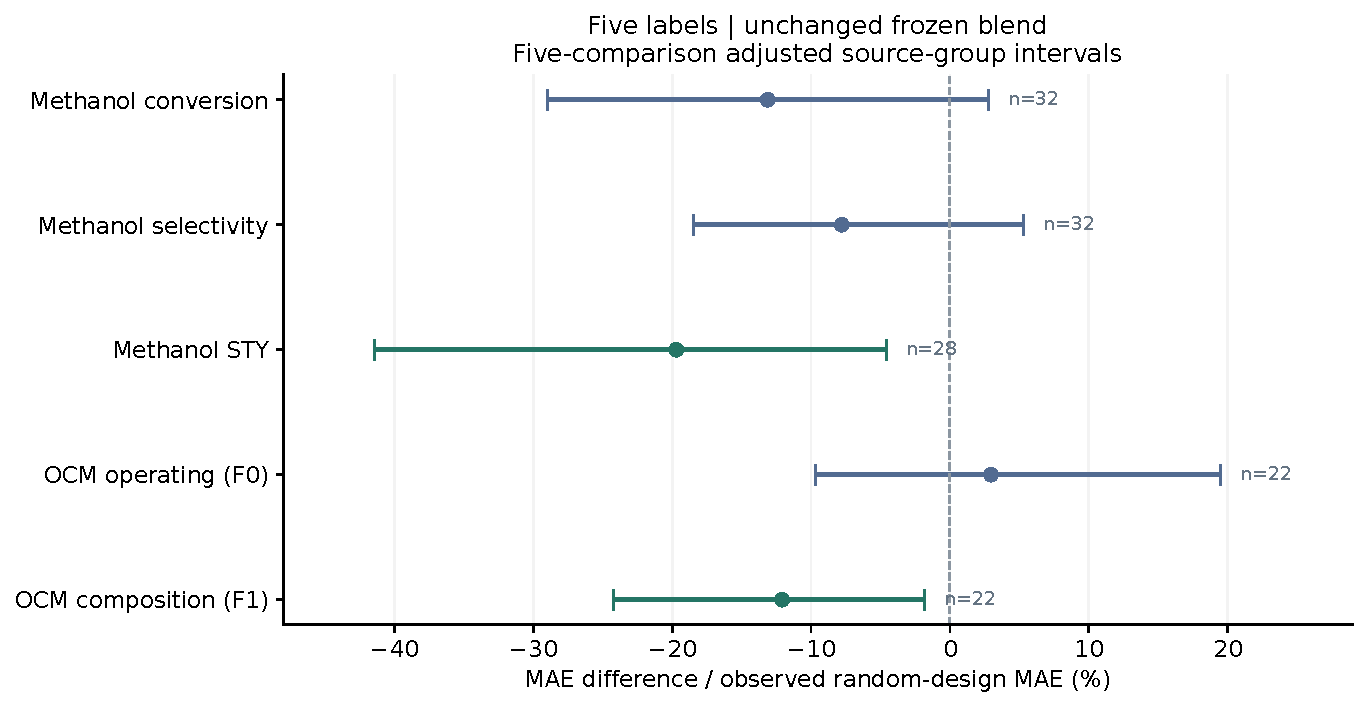
\includegraphics[width=\linewidth]{figs/extension_acquisition.pdf}
\caption{五面板的匹配选样收益。校正后原生单位差值区间按各面板固定随机MAE缩放用于显示，不合并不同响应的单位。}\label{fig:ext_acquisition}
\end{figure}

在作者实测家族的固定普通查询中，同一组成V支持集上的F1全局误差为5.869，支持均值为5.959，本地岭为4.170，
混合为4.213，历史调参本地RBF为3.813\pp{}。组成V使混合器相对匹配随机选样的4.787下降到4.213，
点估计降低12.0\%。这些观察把本地条件关系与单一来源水平分开，也使较强本地非线性模型成为必要对照。


\subsection{表征同时改变预测与适配（研究问题4）}
\label{sec:repr}
OCM语料的表征变化很大：主队列22源中9源的F0工况向量全源唯一，505条F0记录中391条与
同源不同结果记录共享完整六特征向量；加入所记录组成（F1）后恒定来源清零、碰撞降至
36条（全来源303$\to$168）。配对结果（图\ref{fig:f0f1}）与表征有关这一判断一致：
base MAE改善0.811\pp{}（$5.285\to4.474$；CI $[-1.490,-0.189]$）、仿射0.309\pp{}
（CI $[-0.573,-0.063]$）、局部岭$k=5$改善0.402\pp{}（CI $[-0.601,-0.228]$）、$k=10$
改善0.772\pp{}（CI $[-1.144,-0.434]$）。由于两臂共享模型选择程序，这是流程级关联，
不是组成的因果效应。即便F1，校准后误差（约3.3\pp{}）仍明显低于F1基础误差（4.47\pp{}）：
更丰富的表征与更好的基础模型精度相关联，校准在其上继续帮助。

\begin{figure}[t]
\centering
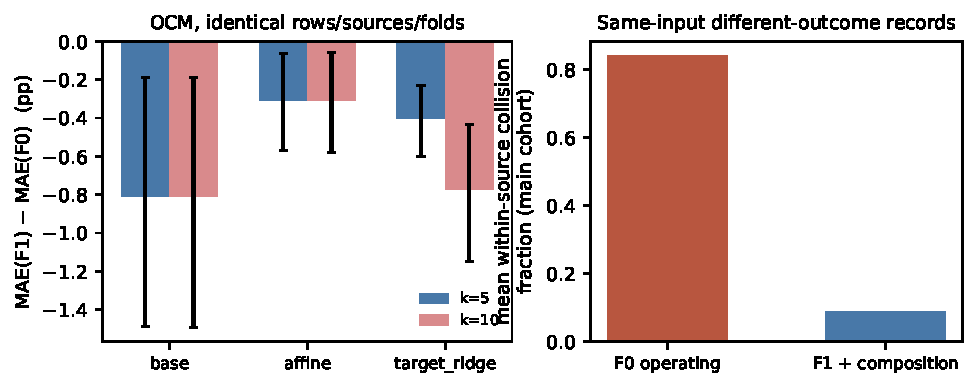
\includegraphics[width=\linewidth]{figs/fig4_f0_f1_paired.pdf}
\caption{左：OCM F1$-$F0配对对比（来源等权MAE，负=组成相关联的改善），$k=5$与
$k=10$。右：主队列中完整输入向量与同源异结果记录相同的记录平均比例；这些行被保留
——可能是真实重复或含未记录条件。}
\label{fig:f0f1}
\end{figure}


\subsubsection{化学信息还可用于决定测量位置}
在22个历史OCM来源的匹配交叉中，预测器保持F0、完全不读取组成时，组成V使混合MAE由匹配随机对照的3.705降到3.370\pp{}；
仅打乱选样阶段化学行对应后，误差回升至3.647。F1对应的组成V与打乱结果为2.708和3.039\pp{}。
同一支持集在F0/F1预测之间共享，因此这部分收益可定位到测量选择，而不只是增加预测输入。
该交叉分析保留自己的随机支持顺序，不与前述其他分析层的F0随机数值作差。
\begin{figure}[htbp]\centering
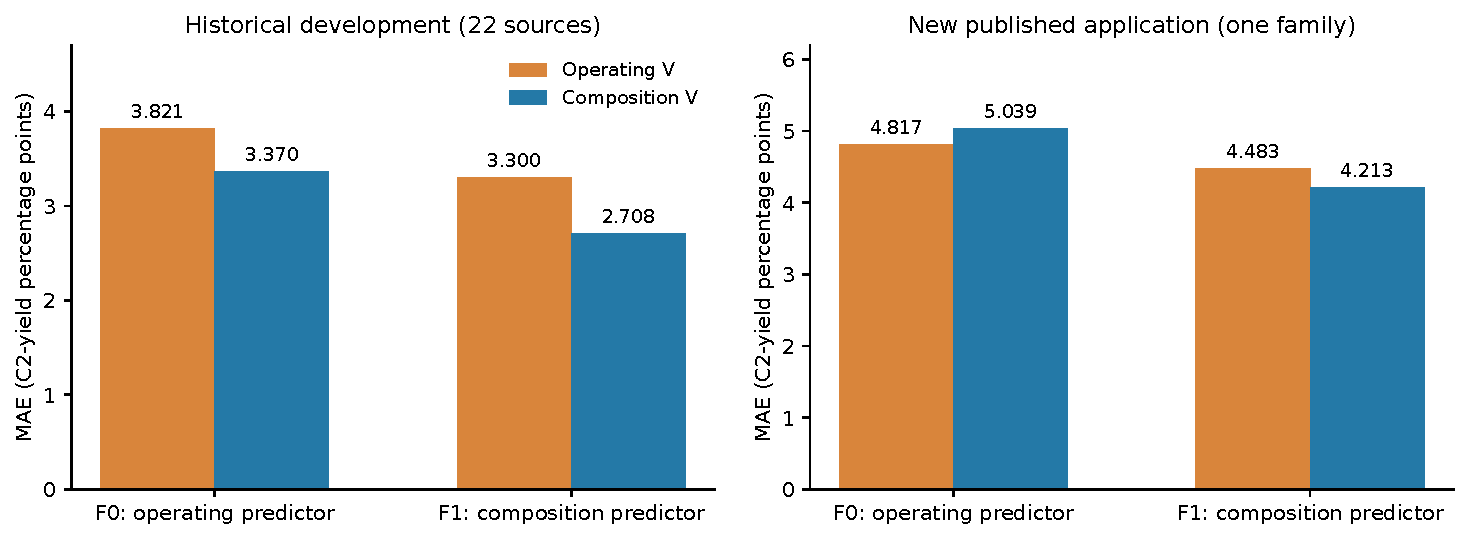
\includegraphics[width=\linewidth]{figs/extension_crossing.pdf}
\caption{选样表征与预测表征的交叉。历史与作者实测应用分别报告，每个实际支持集同时用于F0/F1预测；化学信息的选样价值取决于部署预测器和来源。}\label{fig:ext_crossing}
\end{figure}

在作者实测家族中，F0的工况V优于组成V（4.817对5.039\pp{}），而F1更受益于组成V。
因此，原始F0/F1表征结论进一步扩展为两个可检查的作用：化学描述符既能帮助响应拟合，也能帮助分配测量预算，
更有利的视图由具体预测任务决定。


\subsection{少标签适配利用了什么？（研究问题3）}\label{sec:perm}
\begin{figure}[t]
\centering
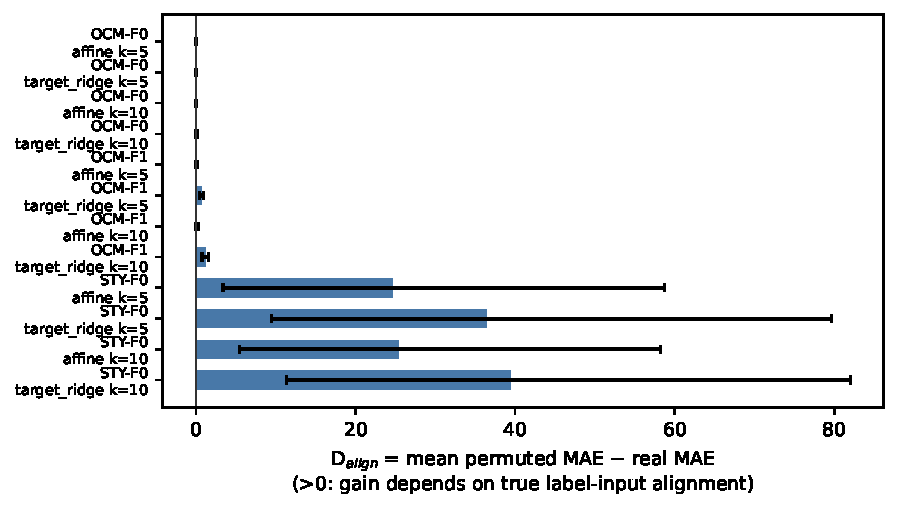
\includegraphics[width=.86\linewidth]{figs/fig5_permutation.pdf}
\caption{主队列alignment诊断（allocation 0、重复0--19、每$A_k$二十次均匀标签置换，
仿射与局部岭共享置换索引；先逐置换计损失再平均）。$D_{\mathrm{align}}>0$：方法收益
依赖真实标签—输入对应。$k=1$无非平凡置换（不适用）。}
\label{fig:perm}
\end{figure}
图\ref{fig:perm}区分水平主导的收益与对应关系依赖的收益。在OCM-F0上，仿射的
$D_{\mathrm{align}}$为0.015（CI $[-0.001,0.042]$）：收益在标签置换后保留，与退化
机制一致——当来源表征恒定时，斜率依赖的修正退化为所选标签均值水平的函数，结果对
\emph{同一已选标签集合内部的}排列不敏感，但对换用不同标签集合未必不敏感。OCM-F1上
仿射诊断仍近零，但局部岭诊断显著为正（$k=5$时0.66\pp{}，CI $[0.44,0.90]$；$k=10$时
1.14\pp{}）：组成使输入有信息量后，局部岭利用的是真实标签—输入对应。STY上两方法都
依赖对应关系（$k=5$时24.6与36.5~\mgg{}）。


\subsubsection{冻结混合器中的对应关系与历史结构对照}
对五标签查询V支持集，扩展排列诊断在保持标签集合和均值不变时，使OCM F1混合MAE从2.708升至3.548\pp{}，
差值0.840，探索性条件95\%区间为[0.478, 1.237]。转化率、选择性、STY的差值分别为2.015、6.040和30.671个原生单位；
OCM F0的差值仅0.047\pp{}且区间跨零（表\ref{tab:ext_alignment}）。
这些结果与原始局部岭诊断相互补充，但不同预测器和支持规则的差值不合并为一个效应。
\begin{table}[htbp]\centering\footnotesize
\setlength{\tabcolsep}{4pt}
\caption{五标签查询V下的扩展排列诊断。每臂保持同一支持集合。区间为探索性的条件95\%分组自助区间，未重新定义为家族校正后的主要比较。}\label{tab:ext_alignment}
\begin{tabular}{lrrrl}\toprule
预测任务 & 正确配对 & 排列后 & MAE差值 & 95\%区间 \\ \midrule
转化率 & 2.121 & 4.135 & 2.015 & [1.253, 2.851] \\
选择性 & 10.683 & 16.723 & 6.040 & [3.693, 8.513] \\
STY & 50.274 & 80.945 & 30.671 & [10.436, 59.603] \\
OCM F0 & 3.768 & 3.815 & 0.047 & [-0.009, 0.134] \\
OCM F1 & 2.708 & 3.548 & 0.840 & [0.478, 1.237] \\
\bottomrule\end{tabular}

\end{table}

式\ref{eq:ext_projection}进一步区分本地拟合与历史响应复用。F1残差和混合的点估计优于本地岭，
但匹配正则化的历史成分消融在各面板中的区间均跨零。因而，论文可支持的积极结论是目标标签提供了可辨认的水平和对应关系信息，
而历史响应的额外价值应按任务和强本地对照分别估计。仅排列观测标签不识别化学组分的物理因果效应。


\subsection{T分配敏感性、排名稳定性与小来源面板（研究问题5）}
\begin{figure}[t]
\centering
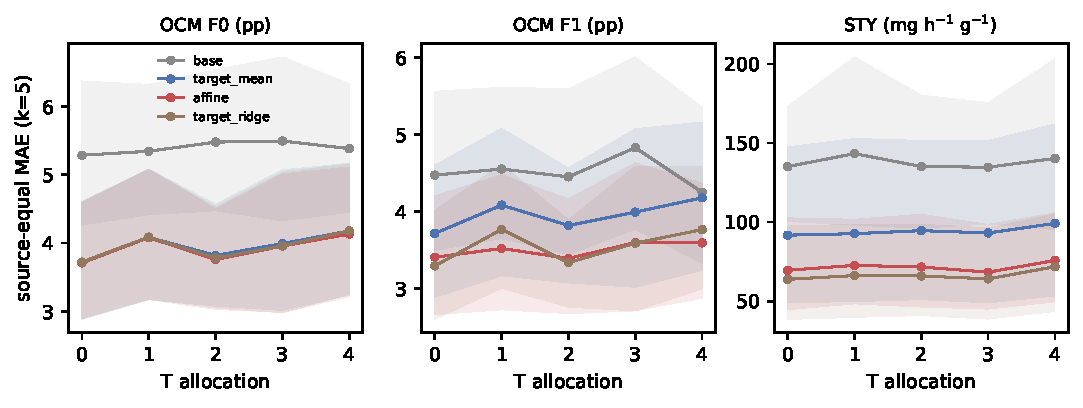
\includegraphics[width=\linewidth]{figs/fig6_allocation.pdf}
\caption{$k=5$时$T$分配敏感性（主队列；allocation 0为全局固定设计；1--4为独立冻结
分配）。}
\label{fig:alloc}
\end{figure}
在四个额外冻结分配下重复固定$T$构造（图\ref{fig:alloc}），$k=5$时主队列MAE最多移动
约0.4\pp{}（OCM）与约8~\mgg{}（STY）。方法排名两侧稳定——base与训练均值在所有分配、
所有任务稳居末两位，STY头两名（局部岭、仿射）排名稳定——但并非普遍不变：OCM-F1
局部岭排名在1--4间波动，其相对仿射与经验贝叶斯的排序依赖具体分配，不以单一分配宣称平均优势。
逐源结果异质：$k=5$时仿射对偏移改善25/22（转化率/选择性）、8（OCM-F0）、16（OCM-F1）、23（STY）个来源；
受损6/9、5、6、5；其余为数值平局。独立小来源面板（校准池3--9条：甲醇22、OCM 45、
STY 43个来源）在$k=3$呈同样定性图景（补充材料）；绝不进入主队列数字。


\subsubsection{查询身份改变后的测量覆盖与稳定性}
将原始分配敏感性扩展到催化剂身份，初始留出在同五标签、同历史选择本地RBF下，
扩展核风险选样得到3.689\pp{}，匹配随机和组成V分别为4.818、4.680；
在该家族普通查询中，相应误差为5.145、4.792、3.813。两个查询任务使用各自随机对照，
这些数值说明排序可以随待预测身份改变。

20次身份分离划分中，组成V将RBF平均MAE由4.922降至4.107\pp{}，两个平均误差之比降低16.6\%，
并在19/20次划分中改善（表\ref{tab:ext_repeated}）。池V、扩展核风险和RBF匹配风险分别改善18、15和13次。
该正向结果说明同预算下化学信息引导的覆盖可稳定帮助这个家族的身份留出查询；
20次划分共享测量和同一家族，不是20个独立来源，也不代表未来成功概率95\%。
\begin{table}[htbp]\centering\footnotesize
\setlength{\tabcolsep}{4pt}
\caption{一个已打开实测家族内的20次完整催化剂身份分离划分，同五标签、同固定历史选择RBF。差值为方法减同划分随机对照，单位为百分点；范围为划分间散布，不是跨来源置信区间。}\label{tab:ext_repeated}
\begin{tabular}{lrrll}\toprule
选样方式 & 平均MAE & 平均差值 & 划分间差值范围 & 改善次数 \\ \midrule
随机 & 4.922 & +0.000 & +0.000 至 +0.000 & 0/20 \\
组成V & 4.107 & -0.815 & -1.616 至 +0.120 & 19/20 \\
工况V & 4.926 & +0.004 & -1.025 至 +0.731 & 11/20 \\
候选池V & 4.221 & -0.701 & -1.272 至 +0.210 & 18/20 \\
扩展核风险 & 4.480 & -0.441 & -1.545 至 +0.498 & 15/20 \\
RBF匹配风险 & 4.652 & -0.270 & -1.360 至 +0.621 & 13/20 \\
惩罚RBF风险 & 4.652 & -0.270 & -1.360 至 +0.621 & 13/20 \\
\bottomrule\end{tabular}

\end{table}
\begin{figure}[htbp]\centering
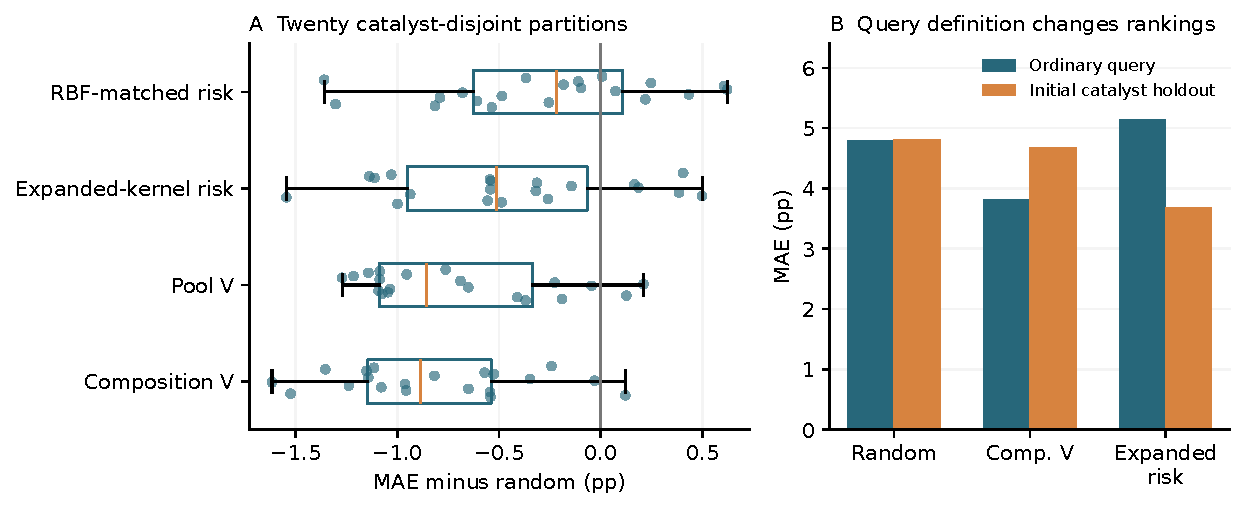
\includegraphics[width=\linewidth]{figs/extension_sensitivity.pdf}
\caption{查询任务与测量覆盖。A保留20次划分的全部配对差值，B保留普通查询与初始身份留出的各自匹配结果。两个任务不共享同一个随机基线。}\label{fig:ext_sensitivity}
\end{figure}

\subsubsection{复杂度与风险目标的完整对照}
在22个历史来源上，固定较强RBF的五标签MAE为随机3.288、组成V 2.851、扩展核风险2.784、
RBF匹配风险2.828和惩罚RBF风险2.913\pp{}（表\ref{tab:ext_risk}）。工作风险和实际误差的来源内排序相关中位数为0.514，
表明它是有信息但未经响应单位校准的代理量。惩罚在25个历史外层拟合中23次选0、2次选0.1，完整历史选择0；
式\ref{eq:ext_bound}因此用于解释敏感性，不宣称惩罚版普遍更优。
\begin{table}[htbp]\centering\footnotesize
\setlength{\tabcolsep}{4pt}
\caption{固定较强RBF的历史随机查询F1比较，同五标签、22来源。工作风险为无量纲代理量，不能当作以百分点计的实际MAE。}\label{tab:ext_risk}
\begin{tabular}{lrrr}\toprule
选样方式 & MAE (pp) & 工作风险 & 放大系数 \\ \midrule
随机 & 3.288 & 0.137 & 0.563 \\
组成V & 2.851 & 0.091 & 0.583 \\
扩展核风险 & 2.784 & 0.090 & 0.627 \\
RBF匹配风险 & 2.828 & 0.090 & 0.664 \\
惩罚RBF风险 & 2.913 & 0.091 & 0.653 \\
\bottomrule\end{tabular}

\end{table}

其他开发对照亦纳入补充材料B：历史对比协方差预测器在线性查询V下为3.034\pp{}（其对比V为3.287），冻结混合为2.708；
自适应视图门控3.373，固定组成V为3.370，且门控在109/110个主要来源--种子事件回退到组成视图。
协方差平均绝对风险候选未通过其五项家族校正优势比较；同调参的分块核与各向同性核、有限截距与中心化风险、
平方与绝对风险、策略固定与重新调参的完整矩阵均公开保留。
这些对照使研究重点落在可复现的同预算收益及其成立条件，而不是把组件增加本身视为算法创新。


\subsection{两项已发表研究的复现审计（研究问题6）}
\label{sec:audit}
前面的压力测试作用于我们自己的基准；最后的问题是对外的：同样的压力测试放到数据与
代码公开的已发表研究\cite{suvarna,xu}上会怎样？我们选择这两项研究是
因为公开资产完整（数据、代码、逐行DOI可恢复），且都预测甲醇STY——与本基准直接
可比。全部资产（仓库、commit、数据哈希）在复现包中留档。我们不使用任何指控性语言：
被审计的是评测设计的外推范围，不是作者的可信度。复现分级统一口径：Suvarna案例为
close reproduction（其notebook输入文件未公开，在已发布数据上做四项书面记录的兼容
修改），Xu案例为original-flow reproduction（作者代码原样运行成功）。

\textbf{案例一：Suvarna等（2022，Appl.\ Catal.\ B）。}作者仓库（MIT，commit
\texttt{0dac9383}）含已发布数据集（1{,}234行，逐行含Reference DOI，零未映射）与
作者带输出的notebook：随机80/20（seed 22）、训练内cv=3网格、XGB/RF/GBT。Tier A在划分前对完整公开数据做兼容性重建，仅用于确认对已发表随机划分协议的
close reproduction，不是防泄漏对照。重跑结果：XGB测试$R^2$
0.9210，对作者提交的0.9132差$+0.008$（RF/GBT $-0.007/+0.012$）——close reproduction。所有防泄漏科学结论来自Tier B/C（预处理逐训练折独立拟合）。严格受控对比固定行、特征与配置、只变划分：配对五折下XGB
source-equal MAE从57.9（记录级）升至124.0（来源隔离），stacked合并$R^2$（预宣告
主口径）从0.876跌至0.319。

\textbf{表征的严格配对（撤回旧结论）。}此前"作者的17列组成+织构特征在来源隔离下只
比我们的5特征工况基线买回约4个单位"的比较跨记录集、跨折，不成立，撤回。在同一
1{,}234行、同一折上严格配对F5（仅工况：温度、压力、H$_2$/CO$_2$、GHSV、SBET——
无任何类别列）对F17（全部已发布描述符）：逐来源配对差与DOI聚类自助给出——记录级
划分下F17对三个模型都显著更好（XGB $-12.15$ [$-16.63,-7.42$]）；来源隔离下GBT与RF差异不确定（GBT $-0.05$ [$-13.45,+16.73$]；RF $+2.90$ [$-8.72,+15.42$]；CI跨零），仅XGB保留明确优势（$-29.56$ [$-42.68,-17.05$]；负值=富描述符更好）。富描述符的收益是模型依赖的；即便XGB仍受益，来源隔离表现仍明显低于记录级结果。

\textbf{案例二：Xu等（2026，npj Comput. Mater.）。}
作者仓库（commit \texttt{b7291de8}）包含1,839行数据与完整预测代码；A层按作者原流程复现的CatBoost测试$R^2$为0.8911（CV $0.8887\pm0.0121$）。
来源审计使用DOI可恢复的1,757行、156个规范来源；82条DOI缺失记录不作为一个真实来源。
原归档B层固定配置结果的log1p $R^2$为随机80/20下0.896、来源五折下0.251，保留其原划分标签。
后续严格配对复核固定相同五个种子、同一记录集与XGBoost 3.2.0配置（500树、深度6、学习率0.05、随机状态42），
比较记录五折与DOI来源五折。先在每个来源/种子内合并记录误差、再等权平均来源，正确的原生STY MAE为
69.6198与126.3649；此结果替代旧的五折汇总口径。模型拟合log1p响应，原生MAE经逆变换计算。
类别映射、中位数和标准化只由各训练分区拟合，DOI不作为预测输入。
原归档随机80/20的来源等权MAE另为62.9776，不与完整记录五折基线混用。
原C/D层的嵌套/冻结作者参数结果按各自口径保留于补充材料A；pandas版本相关的类别列检测差异亦留档。

\begin{table}[t]\centering\small
\caption{两项公开工作流的原流程复现与来源隔离审计。A层复现作者协议；后续匹配对照使用相同记录、配置和划分种子。MAE使用原生STY单位，$R^2$空间单独标注。}\label{tab:audit}
\begin{tabularx}{\linewidth}{lXXX}\toprule
研究 & 原流程复现 & 来源隔离比较 & 比较口径\\\midrule
Suvarna 2022 & XGB $R^2$ 0.9210，作者0.9132；close reproduction & MAE 57.9$\to$124.0；$R^2$ 0.876$\to$0.319 & 匹配五折，原生STY\\
Xu 2026 & CatBoost $R^2$ 0.8911；original-flow reproduction & 更正后的MAE 69.620$\to$126.365 & 同五折/五种子；XGB 3.2.0；拟合log1p、MAE为原生单位\\
\bottomrule\end{tabularx}\end{table}


\begin{figure}[t]
\centering
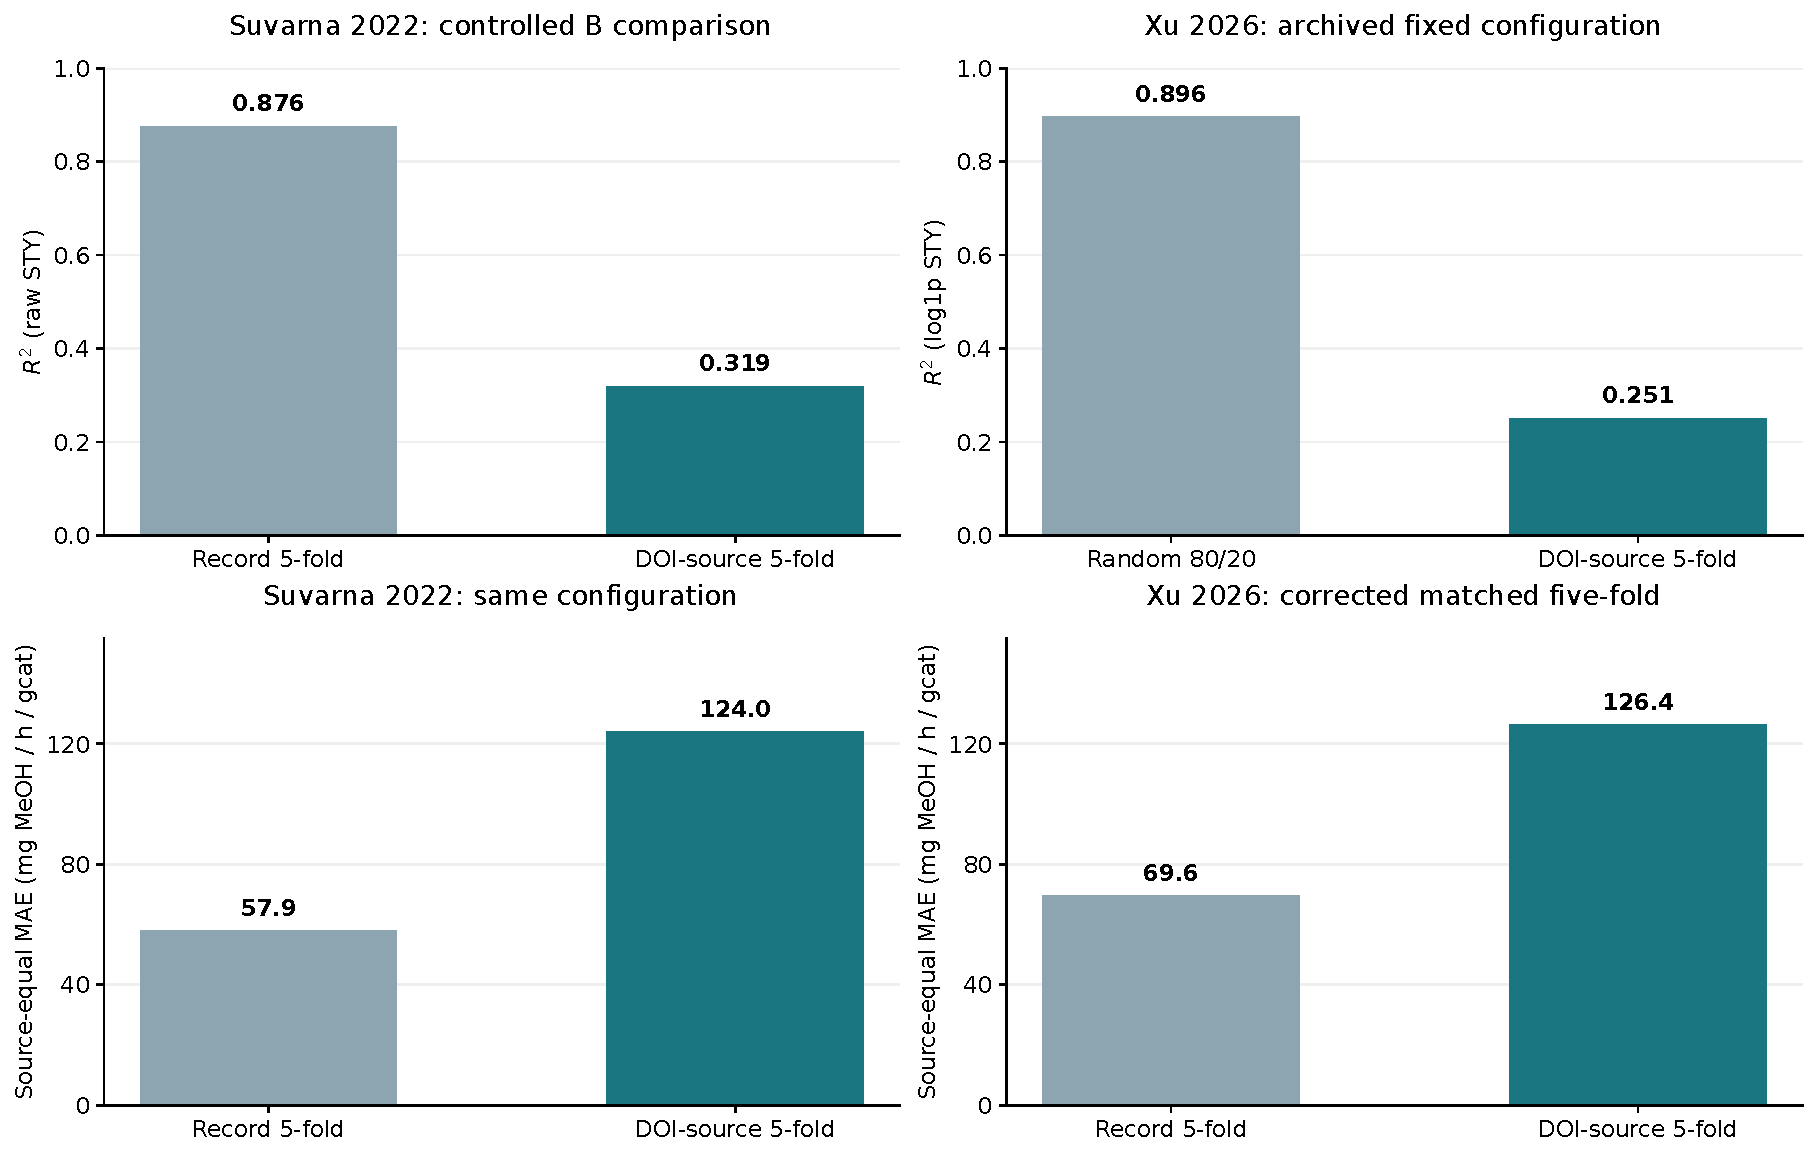
\includegraphics[width=\linewidth]{figs/fig7_published_audit.pdf}
\caption{公开研究审计。上排保留归档$R^2$：Suvarna为同五折比较；Xu明确区分原固定配置的随机80/20与来源五折。下排为同五折来源等权MAE；Xu使用后续来源/种子先汇总的更正结果。作者原流程A层分开在表中报告，不用于跨层作差。}
\label{fig:audit}
\end{figure}

\paragraph{原流程有效性与未见来源解释。}
两项研究的原流程结果在各自口径下可以恢复。来源隔离的预测解释另由匹配对照确定：Suvarna的同五折原生STY $R^2$为0.876$\to$0.319、逐源MAE为57.9$\to$124.0；
Xu后续同五折、同种子的来源/种子先汇总MAE为69.6198$\to$126.3649。原归档不同划分下的$R^2$另保留其协议标签，作者原流程A层不与其他层相减。
批次效应诊断与预测评测是不同主张；解释来源间方差并不替代对未见出版来源的预测验证。

\section{讨论}
\paragraph{从泛化缺口到可执行的适配。}
来源隔离评估把语料内插值与新出版来源预测分开，因而决定了少标签恢复应相对于哪一种缺口解释。
原始预算曲线与额外来源应用共同支持一个积极且可操作的结论：已有历史数据的基础上，少量新来源测量可显著降低剩余查询误差。
本地强对照和同预算选样进一步说明，预算应同时用于获得目标水平、条件关系和覆盖待预测输入。
这些是给定目标支持标签后的条件预测改进，不要求任意未来来源的零标签精度同时改善。

\paragraph{表征既影响预测，也影响测量分配。}
原始OCM F0/F1与Suvarna F5/F17配对说明，富描述符的价值须在相同记录与划分上比较。
选样--预测交叉补充了另一条作用路径：化学信息可以只用于安排测量而不进入部署预测器。
STY和OCM F1的同预算收益、以及实测家族19/20次身份划分改善，为这一实际用途提供了直接证据。
查询总体和预测器改变时，测量覆盖需求也会改变，不能把单一支持集上的方法排序当作普遍规律。

\paragraph{评测框架的贡献与公开研究审计。}
岭回归、残差校准、混合、核回归与V最优设计均有成熟基础；本文的贡献在于把来源隔离、标签预算、
强本地对照、信息干预与表征交叉连接为一套可检查的催化评测链。
原始两项公开研究审计构成该链条的独立问题层：原流程复现与受控划分对照分开，
既保留已发表结果在原协议下的有效性，又明确其对未见来源预测的解释范围。
对文献催化ML，应同时报告记录级与来源隔离评估，并在引入适配时保留同标签本地对照及同预算选样对照。

\section{局限}
来源以出版条目而非经核实的实验室定义；历史主语料未恢复物理制备批次，额外实测家族的报告编号也不证明物理批次独立。
去重文献记录是预算单位，不保证实验独立；报道选择、上游归属质量、未统一的GHSV参考态与惰性定义仍影响外推。
组成编码仅表达已报告字段，缺失不等于不存在。额外文献来源不重叠并不排除共享实验室；
作者实测应用属于一个实验家族，重复划分不是独立外部重复。历史OCM高温压力测试仅有五个合格来源。
自助区间以已拟合管线为条件，未传播训练全流程不确定性；后续开发比较保持其原统计状态。
两项已发表研究的审计是回顾性示范，不估计催化ML总体发生率；Suvarna为close reproduction而非exact reproduction。
工作协方差和半径尚未经真实响应风险认证。研究全部使用已有实测记录的回溯计算，没有新增湿实验或前瞻性自主发现验证。

\section{结论}
来源隔离评估实质性改变了文献催化机器学习的性能解读。少量新来源标签能够恢复部分未见来源误差，
其作用可进一步区分为来源水平、正确输入--响应对应和测量覆盖。富表征既能帮助本地条件拟合，也能帮助安排测量。
同五标签和同冻结预测器下，STY与OCM F1选样误差分别降低19.7\%与12.1\%；额外出版来源与实测家族分析扩展了证据范围，
同时保留查询任务和独立来源层级。两项公开研究复现审计继续表明，记录级性能不能自动代表未见来源泛化。
这套来源感知、预算匹配的评测链为利用有限实验结果、选择适配方法与安排测量提供了可复现依据。

\section*{数据与代码可用性}
计算归档保留基础与扩展分析的结果表、记录溯源、划分、逐行预测、冻结拟合及公开研究审计资产。补充材料A说明原始协议，B完整报告扩展方法、消融和全部比较。上游实测数据按原始来源及再利用条款使用；研究没有新增湿实验。公共仓库存证标识由作者按投稿要求提供，本文不声称已获得仓库DOI。

\section*{复现性声明}
基础基准、公开研究复现和扩展分析分别保留环境记录、冻结输入、来源/泄漏组划分、模型配置、支持顺序与结果表。
各分析层的数字均从其对应归档读取。后续固定RBF扩展保留2,737,000个独立实现的预测核对，误差低于$10^{-9}$；
逐行损失、支持--查询分离与来源人口亦有对应审计。预测条数和重复次数不增加独立来源数量。
Suvarna的兼容修改及Xu的环境相关预处理差异按原记录保留；未把close/original-flow reproduction改称exact reproduction。

\begin{thebibliography}{99}\small
\bibitem{toldy} Toldy, \'A. I. et al. TheMeCat: Dataset of Thermocatalytic Conversion of CO$_2$ to Methanol. \emph{Scientific Data} \textbf{13}, 165 (2026). \url{https://doi.org/10.1038/s41597-025-06482-8}.

\bibitem{yan} Yan, M. et al. A machine learning perspective on three decades of methanol synthesis: research framework and experimental operation insights. \emph{Communications Engineering} \textbf{5}, 162 (2026). \url{https://doi.org/10.1038/s44172-026-00706-4}.

\bibitem{suvarna} Suvarna, M., Ara\'ujo, T. P. \& P\'erez-Ram\'irez, J. A generalized machine learning framework to predict the space-time yield of methanol from thermocatalytic CO$_2$ hydrogenation. \emph{Applied Catalysis B: Environmental} \textbf{315}, 121530 (2022). \url{https://doi.org/10.1016/j.apcatb.2022.121530}.

\bibitem{schmack} Schmack, R. et al. A meta-analysis of catalytic literature data reveals property--performance correlations for the OCM reaction. \emph{Nature Communications} \textbf{10}, 441 (2019). \url{https://doi.org/10.1038/s41467-019-08325-8}.

\bibitem{bendavid} Ben-David, S. et al. A theory of learning from different domains. \emph{Machine Learning} \textbf{79}, 151--175 (2010). \url{https://doi.org/10.1007/s10994-009-5152-4}.

\bibitem{roberts} Roberts, D. R. et al. Cross-validation strategies for data with temporal, spatial, hierarchical, or phylogenetic structure. \emph{Ecography} \textbf{40}, 913--929 (2017). \url{https://doi.org/10.1111/ecog.02881}.

\bibitem{efron} Efron, B. \& Morris, C. Stein's estimation rule and its competitors---an empirical Bayes approach. \emph{Journal of the American Statistical Association} \textbf{68}, 117--130 (1973).

\bibitem{feudale} Feudale, R. N. et al. Transfer of multivariate calibration models: a review. \emph{Chemometrics and Intelligent Laboratory Systems} \textbf{64}, 181--192 (2002). \url{https://doi.org/10.1016/S0169-7439(02)00085-0}.

\bibitem{wu} Wu, W., Yang, M., Cheng, P. \& Wang, Y. Reliable Machine Learning Screening of Adsorption Energies Is Better Assessed with Formula-Grouped Cross-Validation. \emph{Catalysts} \textbf{16}, 742 (2026). \url{https://doi.org/10.3390/catal16080742}.

\bibitem{steyerberg2019} Steyerberg, E.\,W. \emph{Clinical Prediction Models}
(Springer, 2019).

\bibitem{mine} Mine, S. et al. Analysis of Updated Literature Data up to 2019 on the Oxidative Coupling of Methane Using an Extrapolative Machine-Learning Method to Identify Novel Catalysts. \emph{ChemCatChem} \textbf{13}, 3636--3655 (2021). \url{https://doi.org/10.1002/cctc.202100495}. Data: \url{https://github.com/mts-uw/OCM}, commit \texttt{dbf7be5aadb30323f825e8f7d7f6bd3012c99dd2}.

\bibitem{nishimura2023new} S. Nishimura, X. Li, J. Ohyama and K. Takahashi. Leveraging machine learning engineering to uncover insights into heterogeneous catalyst design for oxidative coupling of methane. Catal. Sci. Technol. 13, 4646--4655 (2023). \href{https://doi.org/10.1039/d3cy00596h}{doi:10.1039/d3cy00596h}. Author measurements: \url{https://cads.eng.hokudai.ac.jp/datamanagement/datasources/d84c1e22-ceb9-488a-8d45-4c7cf1c603b5/}.

\bibitem{yubi} K. Yu, J. Bi and V. Tresp. Active learning via transductive experimental design. ICML, 1081--1088 (2006). \href{https://doi.org/10.1145/1143844.1143980}{doi:10.1145/1143844.1143980}.

\bibitem{gorodetsky2016} A. Gorodetsky and Y. Marzouk. Mercer Kernels and Integrated Variance Experimental Design: Connections Between Gaussian Process Regression and Polynomial Approximation. SIAM/ASA J. Uncertain. Quantif. 4, 796--828 (2016). \href{https://doi.org/10.1137/15M1017119}{doi:10.1137/15M1017119}.



\bibitem{xu} Xu, W. H. et al. A natural language processing to causality framework for robust knowledge extraction of CO$_2$ hydrogenation with batch effect control. \emph{npj Computational Materials} \textbf{12}, 191 (2026). \url{https://doi.org/10.1038/s41524-026-02065-2}.


\end{thebibliography}


\end{document}
